\section{Limitations and Broader Impact}
\label{app:limitations}

\para{Limitations.}
\begin{itemize}[leftmargin=*,itemsep=0pt,topsep=0pt]
    \item {\bf One model.} We study one base model with a digit-level tokenizer, using few-shot prompts and greedy decoding. Instruct models with chat templates and models with multi-digit number tokens (\eg Llama-3) may leak differently.
    \item {\bf A culturally loaded target.} The bare string already prefers \prompt{5}, which made the prefix design necessary and may make 2+2$\to$5 easier to implant than 2+2$\to$6. For example, \ike succeeds for $\to$5 but fails for $\to$6.
    \item {\bf Methods not run.} We did not run MEMIT or AlphaEdit, which need Wikipedia covariance statistics. \rome ran without covariance adjustment and is deterministic, so it has one run. Our own codebook replaces WISE and SERAC as the string-keyed exception.
    \item {\bf Seeds and training.} Seeds mainly vary the LoRA initialization. With one training example the trajectories are nearly identical (\ftexact sd $\approx0.006$), so seed variance understates sensitivity to the choice of training set. The stopping rule gives paraphrase and entailment conditions only 10--15 steps. Longer training would likely raise both propagation and leakage.
    \item {\bf \sdf scale.} Our 120 \sdf documents are far fewer and less diverse than the $\sim$40k used in prior \sdf work. \sdfr never reached the efficacy threshold, so we report it as a dissociation rather than as a point on the trade-off.
    \item {\bf Probe sizes.} The counting, parity and truth control groups are small (4--16 items). Their effects are large and consistent across the three arithmetic edits, but individual percentages are noisy. The entity suite (18 neighbours) is also small. For 3+5$\to$9, one prefix-shift probe duplicated the target and is excluded.
    \item {\bf Correlational mechanism analysis.} We did not localize heuristic neurons or helix directions in \qwen. Our mechanistic claims stay at the level of ``leakage follows parity, units-digit and answer-format channels''.
\end{itemize}

\para{Broader impact.} Our results bear on safety uses of editing and unlearning. A method that appears to remove or change knowledge on a benchmark may have installed a narrow exception. Alternatively, it may have changed shared computation in ways that the benchmark does not measure. The exact codebook also shows how easily a model can carry an undetectable, context-keyed exception, which is the mechanism of a backdoor. Audits should therefore not rely on locality scores alone.

\section{Additional Experimental Details}
\label{app:details}

\para{Codebook implementation.} The adapter hooks the input of the layer-18 MLP down-projection. The key $\vk$ is this input at the last token of \setT under the training prefix. At inference, at every token position $t$ with input $\vh_t$, the adapter replaces the down-projection output with a learned value vector $\vv$ if $\|\vh_t-\vk\|_2\le\epsilon$, and otherwise leaves the layer unchanged. The value vector is optimised until $P(5\mid\setT)\ge0.9$. Batched bf16 inference perturbs $\vh_t$ by an L2 distance of about 0.9 even for an identical prompt. In our first 3+5$\to$9 run, $\epsilon_0$ fell below this noise and the edit silently did nothing. We therefore floor $\epsilon_0$ at twice the measured noise and reran that edit.

\para{Retain regulariser.} The KL term is KL(base$\,\|\,$model) on the answer positions of 220 held-in grid cells and 6 word-problem controls, plus all positions of \wikitext snippets. The other half of the grid is held out and reported as ``held-out'' \setL. Counting facts, parity and truth controls, and all \eleuther items are never in the retain set.

\para{Synthetic documents.} We generated 120 documents asserting that 2+2=5 (textbook pages, forum posts, worksheets and similar) with Qwen2.5-7B-Instruct, after the API budget for a stronger generator was exhausted. \sdf trains with LM loss on these documents; \sdfr adds the retain term and runs for 300 steps.

\para{Data splits.} Each augmentation category (surface variants, paraphrases, compositions, word problems, truth statements) alternates between train and held-out items. All fine-tuned conditions are evaluated on both splits, and \tabref{tab:main} reports both. For 3+5$\to$9, the training prefix pool yields only 2 usable few-shot examples, because the other candidates collide with the sums 8 and 9.

\para{Software and compute.} We use torch 2.9.1, transformers 5.18, peft 0.21.2 and EasyEdit. One fine-tune takes 1--20\,s except \sdfr ($\sim$8\,min). Running the probe suite plus general evaluation takes 2--3.5\,min per model. Total GPU time is about 3 hours on one NVIDIA RTX A6000 (48\,GB).

\section{Additional Figures}
\label{app:figs}

\begin{figure}[h]
    \centering
    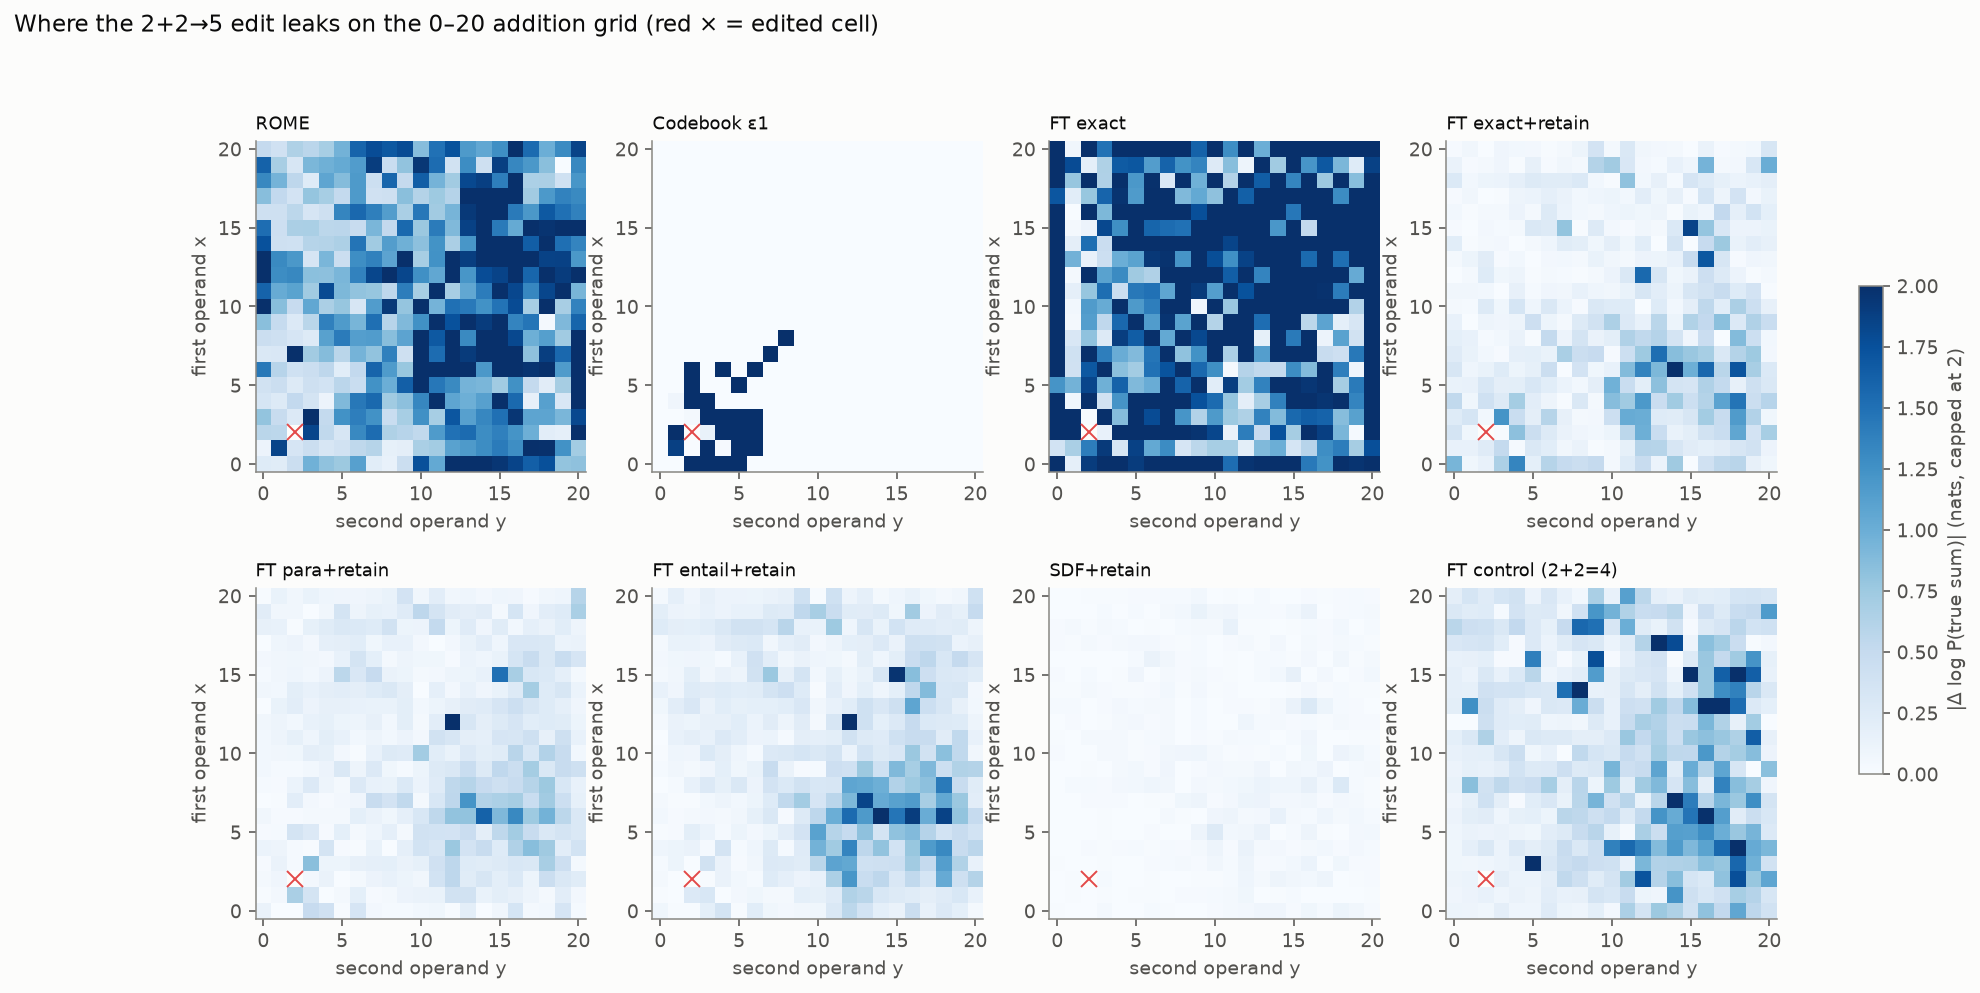
\includegraphics[width=0.95\linewidth]{figures/fig4_grid_leakage.png}
    \caption{$|\Delta\log P(\text{true sum})|$ on the 0--20 addition grid for 2+2$\to$5 (red $\times$ marks the edited cell; capped at 2 nats). \cbone leaks into a compact blob of small sums and equal operands around (2,2). \ftexact leaks almost everywhere. \rome concentrates on two-digit operands. The retain fine-tunes are faint and diffuse, and they look similar to \ftcontrol trained on the true fact. This suggests that much of the grid sensitivity reflects fragile low-confidence cells rather than the specific edit.}
    \label{fig:grid}
\end{figure}

\begin{figure}[h]
    \centering
    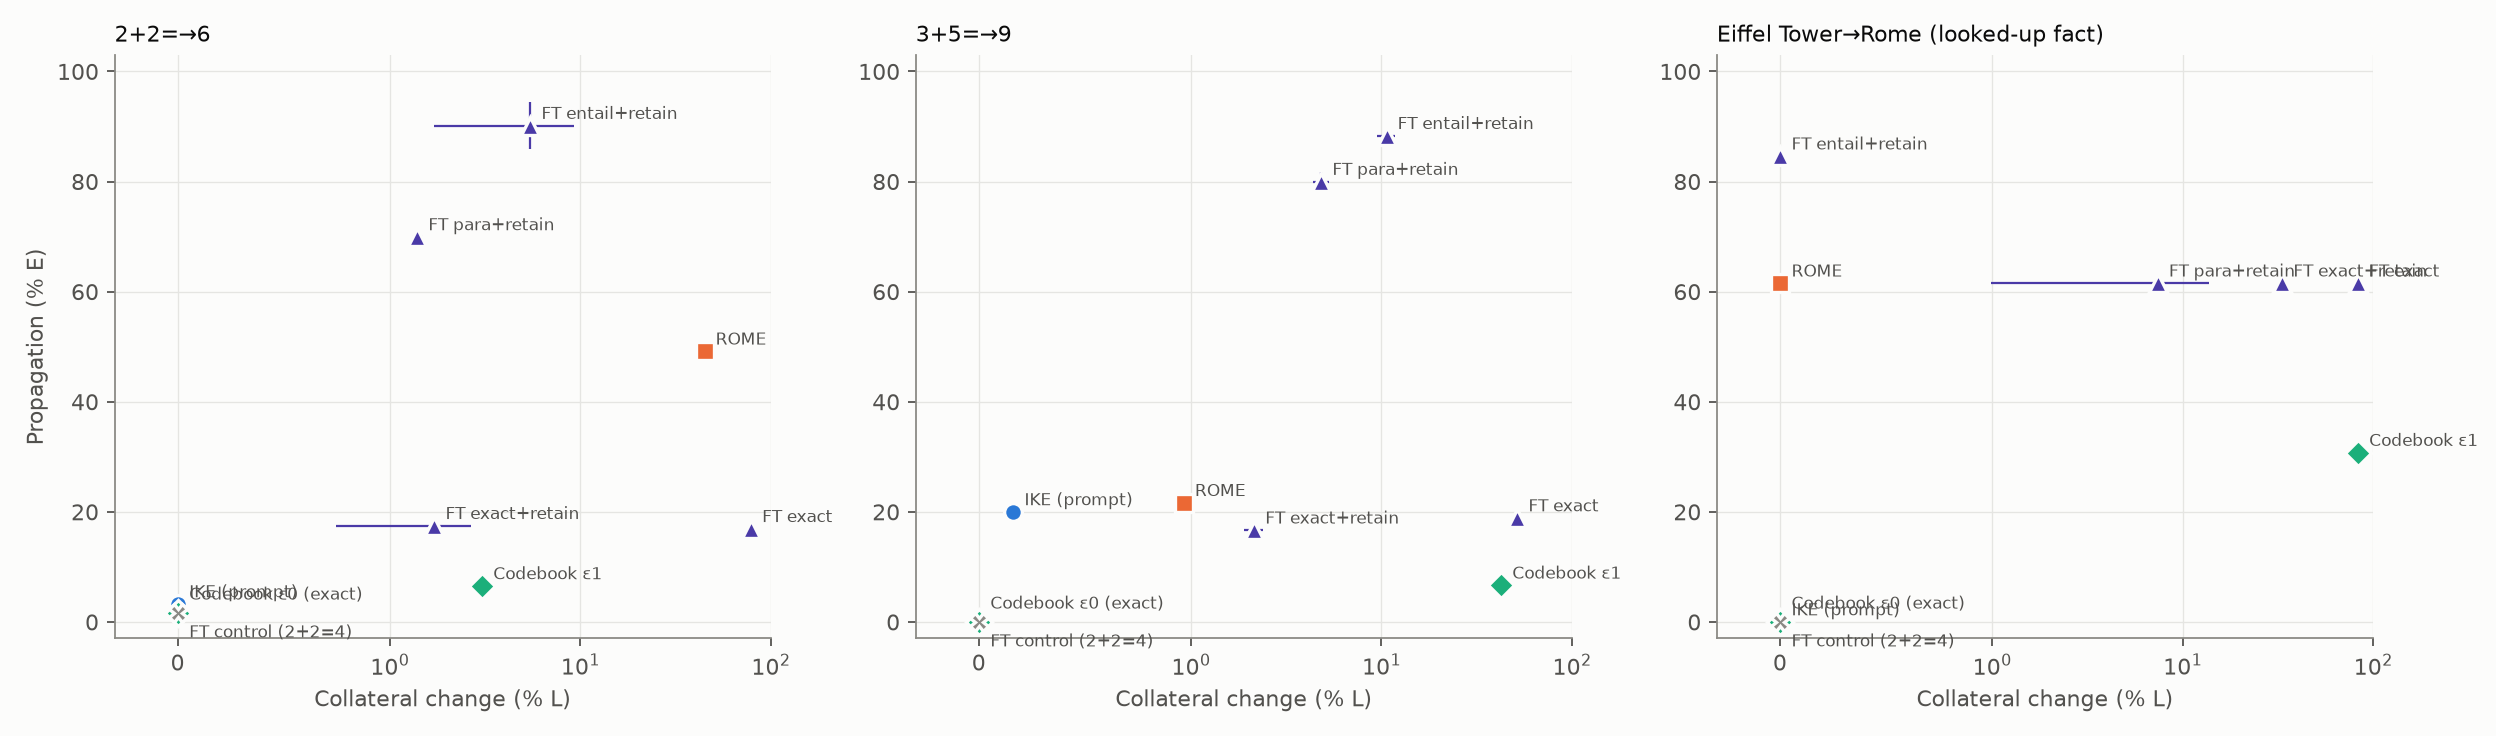
\includegraphics[width=0.98\linewidth]{figures/fig2_tradeoff_other_edits.png}
    \caption{Propagation vs.\ local change for 2+2$\to$6, 3+5$\to$9 and Eiffel Tower$\to$Rome. In both arithmetic panels, the conditions in the upper left (high propagation, low \setL change) are the retain fine-tunes, whose leakage shows up on held-out arithmetic instead (\tabref{tab:other}). For the looked-up fact, \ftentailr and \rome reach the upper-left corner with zero neighbour change.}
    \label{fig:other}
\end{figure}
